\documentclass[../main.tex]{subfiles}

\begin{document}

Most of the state-of-the art image alignment algorithms compare images only considering low-frequency features of the images. It is widely accepted that information beyond $8 \si{\angstrom}$ of resolution is not relevant for the alignment of \gls{cryoem} images. In spite of this, all prior tests were done with a resolution limit of $15 \si{\angstrom}$, as this is closer to the operating range of the algorithm. The aim of this section is to explore how the algorithm behaves across different resolution limits, either below and above the previously considered limit.

\subsubsection{Accuracy}
Figures \ref{fig:5:resolution_angle_accuracy}, \ref{fig:5:resolution_shift_accuracy} and \ref{fig:5:resolution_resolution} show that beyond a resolution limit of $12 \si{\angstrom}$, the alignment accuracy and reconstruction resolution stop improving. This turning point is consistent across all four datasets. However, the actual accuracy value of both angular and shift measurements varies depending on the dataset, likely due to different noise levels. 

Curiously, for simulated images the large angular error induced by missmatched symmetry of the EMPIAR-10256 dataset disappears at this resolution limit. However, this effect cannot be observed for experimental images, as it plateaus at a very high alignment error.

\begin{figure}[htbp]
    \centering
    \begin{subfigure}[b]{.8\textwidth}
         \centering
         \includegraphics[width=\linewidth]{results/resolution/simulated/angle error}
         \caption{Simulated images}
    \end{subfigure}\\
    \vspace{2em}
    \begin{subfigure}[b]{.8\textwidth}
         \centering
         \includegraphics[width=\linewidth]{results/resolution/experimental/angle error}
         \caption{Experimental images}
    \end{subfigure}
    \caption{Angle accuracy in terms of the alignment resolution limit}
    \label{fig:5:resolution_angle_accuracy}
\end{figure}

\begin{figure}[htbp]
    \centering
    \begin{subfigure}[b]{.8\textwidth}
         \centering
         \includegraphics[width=\linewidth]{results/resolution/simulated/shift error}
         \caption{Simulated images}
    \end{subfigure}\\
    \vspace{2em}
    \begin{subfigure}[b]{.8\textwidth}
         \centering
         \includegraphics[width=\linewidth]{results/resolution/experimental/shift error}
         \caption{Experimental images}
    \end{subfigure}
    \caption{Shift accuracy in terms of the alignment resolution limit}
    \label{fig:5:resolution_shift_accuracy}
\end{figure}

\begin{figure}[htbp]
    \centering
    \begin{subfigure}[b]{.8\textwidth}
         \centering
         \includegraphics[width=\linewidth]{results/resolution/simulated/resolution}
         \caption{Simulated images}
    \end{subfigure}\\
    \vspace{2em}
    \begin{subfigure}[b]{.8\textwidth}
         \centering
         \includegraphics[width=\linewidth]{results/resolution/experimental/resolution}
         \caption{Experimental images}
    \end{subfigure}
    \caption{Reconstruction resolution in terms of the alignment resolution limit}
    \label{fig:5:resolution_resolution}
\end{figure}

\subsubsection{Performance}
In contrast to the prior results, the computational cost of the alignment increases rapidly as the resolution limit increases. This is primarily because higher resolution limits involve more reference images. Indeed, we have estimated that the reference count increases with the power of five as the resolution increases.  

\begin{figure}[htbp]
    \centering
    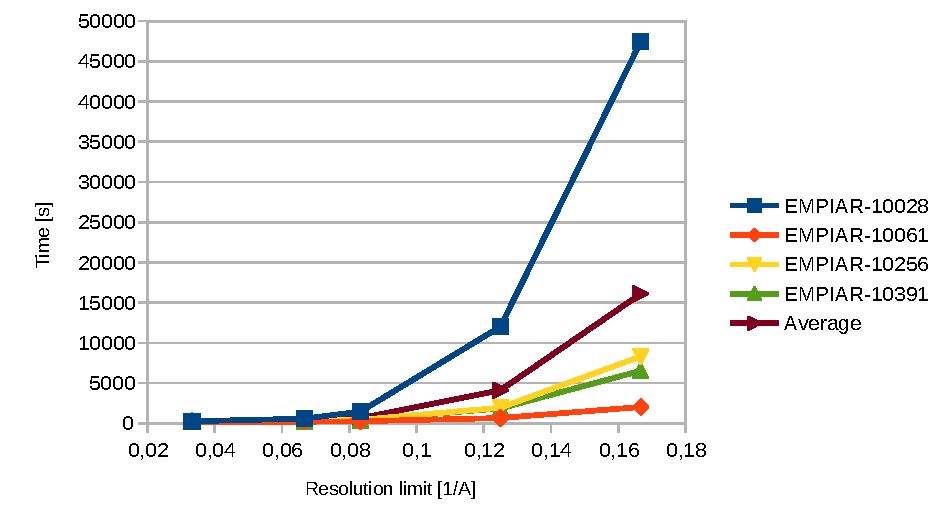
\includegraphics[width=.8\linewidth]{results/resolution/simulated/constant time}
    \caption{Constant time (Training + Populate) in terms of the alignment resolution limit}
    \label{fig:5:resolution_constant}
\end{figure}

\begin{figure}[htbp]
    \centering
    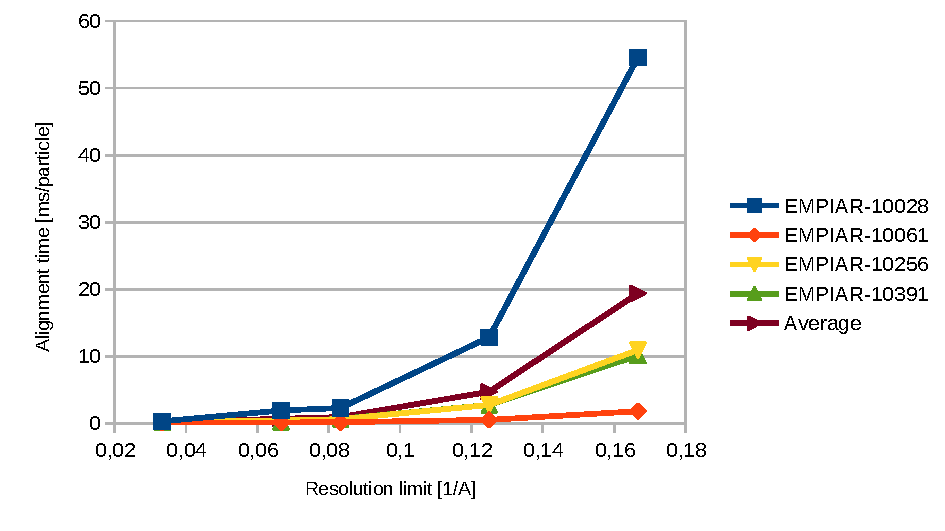
\includegraphics[width=.8\linewidth]{results/resolution/simulated/alignment time}
    \caption{Alignment time in terms of the alignment resolution limit}
    \label{fig:5:resolution_alignment}
\end{figure}

Considering prior measurements, it is important to spare on the resolution limit, as it heavily affects performance but does not provide result improvements beyond a $12 \si{\angstrom}$. In any case, we are researching ways to get closer to the theoretical $8 \si{\angstrom}$ limit in a practical way, so that we can obtain better results.

\end{document}